\begin{problem}[习题4.4]
写出Huffman编码的伪代码, 并编程实现.
\end{problem}
\begin{solution}
\textbf{解:}Huffman编码的伪代码见表\ref{huffmanArithmetic}. 其中函数Extract-Min(Q)是从Q中取出频率最小的节点.
\begin{table}[!htb]
\centering
\caption{\label{huffmanArithmetic}Huffman编码的伪代码}
\begin{tabular}{llll}
\hline
\multicolumn{4}{l}{\textbf{Proc} Huffman(A)\textcolor{blue}{//A为需要编码的字符集}} \\
 & \multicolumn{3}{l}{n = $|A|$;} \\
 & \multicolumn{3}{l}{Q = 按频率分布从小到大排序A} \\
 & \multicolumn{3}{l}{\textbf{for} i \textbf{to} n \textbf{do}} \\
 &  & \multicolumn{2}{l}{z = 新节点} \\
 &  & \multicolumn{2}{l}{left(z) = Extract-Min(Q); \textcolor{blue}{//取出Q中的第一个节点,并从Q中删去}} \\
 &  & \multicolumn{2}{l}{right(z) = Extract-Min(Q); \textcolor{blue}{//取出Q中的第一个节点,并从Q中删去}} \\
 &  & \multicolumn{2}{l}{frequency(z) =  frequency(left(z)) + frequency(right(z))} \\
 &  & \multicolumn{2}{l}{Insert(Q, z); \textcolor{blue}{//向Q中按频率顺序插入新节点}} \\
 & \multicolumn{3}{l}{\textbf{end\{for\}}} \\
 & \multicolumn{3}{l}{\textbf{return} Extract-Min(Q)} \\
\multicolumn{4}{l}{\textbf{end}\{Huffman\}} \\
\hline
\end{tabular}
\end{table}

实现的具体C++代码见附录\ref{sec:Huffman}. 在linux下经g++编译并运行得到图\ref{huffmanResult}.
\begin{figure}[!htb]
\centering
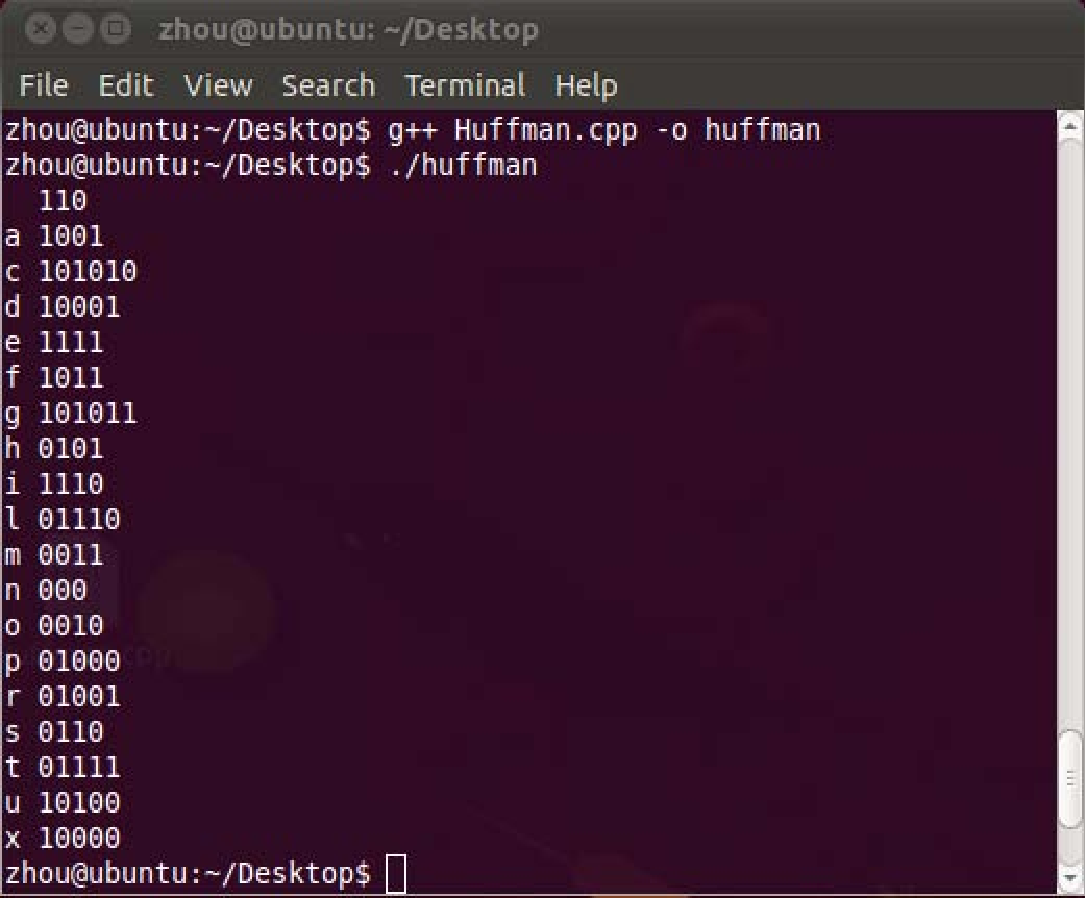
\includegraphics[width=0.7\textwidth]{huffman.pdf}
\caption{\label{huffmanResult}Huffman编码C++程序运行结果}
\end{figure}

\end{solution}
